\section{Theoretical background}

Consider a of 3D gravity or magnetic sources be defined over a closed region 
$\overline{\mathcal{V}'}$ located in the subsurface, with top limited by a vertical 
coordinate $z^{t}_{0}$ in a topocentric Cartesian coordinate system with axes 
$x$, $y$, and $z$ pointing to north, east and down, respectively.
The potential field produced by the 3D sources at observation points 
$\mathbf{r} = (x, y, z)^{\top}$ (Fig.  \ref{fig:Figure1}) is represented by:
\begin{equation}
	d^{o}(\mathbf{r}) = D_{d} \, U(\mathbf{r}) \: , 
	\quad \mathbf{r} \notin \overline{\mathcal{V}'} \: ,
	\label{eq:observed-data-space}
\end{equation}
where $D_{d}$ is a space-domain differential operator acting on the Newtonian potential
\begin{equation}
	U(\mathbf{r}) = \kappa \iiint\limits_{\overline{\mathcal{V}'}}
	\sigma(\mathbf{r}') \: \frac{1}{\| \mathbf{r} - \mathbf{r}'\|}
	\: d\mathcal{V}' \: , 
	\quad \mathbf{r} \notin \overline{\mathcal{V}'} \: ,
	\label{eq:potential-U-space}
\end{equation}
$\kappa$ is a proportionality constant,
$\tfrac{1}{\| \mathbf{r} - \mathbf{r}' \|}$ is the inverse distance function
between the observation point $\mathbf{r}$ and a point 
$\mathbf{r}' = (x', y', z')^{\top} \in \overline{\mathcal{V}'}$
and $\sigma$ is the scalar function representing 
the density (contrast) or total-magnetization intensity within the sources.
\cite{oliveirajr_etal2026_1} propose the following general formula to define the 
space-domain differential operator $D_{d}$ (Eq. \ref{eq:observed-data-space}) 
and its corresponding counterpart $\alpha_{d}$ in the Fourier domain:
\begin{equation}
	D(\ell, \hat{\mathbf{u}}) = 
	\left( \hat{\mathbf{u}}^{\top} \nabla \right)^{\ell} \Leftrightarrow
	\alpha(\ell, \hat{\mathbf{u}}) = \left( \hat{\mathbf{u}}^{\top} \mathbf{k} \right)^{\ell} \: ,
	\quad \ell \in \{ 0, 1, 2 \} \: ,
	\label{eq:diff-operators-generic}
\end{equation}
where $\hat{\mathbf{u}}$ is a constant unit vector,
$\nabla$ is the vector differential operator nabla, 
$\mathbf{k} = ( \mathtt{i} \, k_{x} \, , \, \mathtt{i} \, k_{y} \, , \, k)^{\top}$
\citep{pedersen1978}, $k_{x}$ and $k_{y}$ and represent the wavenumbers along the $x$ and $y$
directions and $k = \sqrt{k_{x}^{2} + k_{y}^{2}}$.
Different potential fields $d^{o}$ (Eq. \ref{eq:observed-data-space}) can be 
defined by properly setting $\ell$ and $\hat{\mathbf{u}}$ in the left side of equation
\ref{eq:diff-operators-generic}. 

Many geophysical applications require the computation of potential-field transformations that convert the
observed potential field $d^{o}$ (Eq. \ref{eq:observed-data-space}) into another potential field 
given by
\begin{equation}
	f(\mathbf{r}) = D_{f} U(\mathbf{r}) \: , 
	\quad \mathbf{r} \notin \overline{\mathcal{V}'} \: ,
	\label{eq:transformed-field-space}
\end{equation}
where $D_{f}$ is a space-domain differential operator 
(Eq. \ref{eq:diff-operators-generic}) acting on $U$ (Eq. \ref{eq:potential-U-space}).
The ``equivalent-layer technique'' is the common approach to compute potential-field transformations
in the space domain and this is usually performed in two steps.
The first consists in estimating a ``continuous equivalent layer'' $p_{\varepsilon}$ 
\citep{oliveirajr_etal2026_1} over a horizontal surface $\mathcal{S}''$ with constant vertical
coordinate $z''_{0}$, so that the predicted potential field
\begin{equation}
	d_{\varepsilon}(\mathbf{r})
	= \int\limits_{-\infty}^{\infty}\int\limits_{-\infty}^{\infty}
	p_{\varepsilon}(\mathbf{r}'') \, D_{a} \Psi(\mathbf{r}, \mathbf{r}'') \:\: d\mathcal{S}''
	\: , \quad z < z''_{0} \: ,
	\label{eq:predicted-data-continuous-layer}
\end{equation}
satisfactorily approximates the observed potential field $d^{o}$ 
(Eq. \ref{eq:observed-data-space}) within a predefined error level,
where $D_{a}$ is a space-domain differential operator 
(Eq. \ref{eq:diff-operators-generic}) acting on the scaled inverse 
distance function between $\mathbf{r}$ and 
$\mathbf{r}'' = (x'', y'', z''_{0})^{\top} \in \mathcal{S}''$ given by
\begin{equation}
	\Psi(\mathbf{r}, \mathbf{r}'') = 
	\frac{1}{2\pi} \: 
	\frac{1}{\| \mathbf{r} - \mathbf{r}'' \|} \: , 
	\quad \mathbf{r} \ne \mathbf{r}'' \: .
	\label{eq:Psi}
\end{equation}
The second step in the equivalent-layer technique involves using the estimated $p_{\varepsilon}$ 
(Eq. \ref{eq:predicted-data-continuous-layer}) to compute the transformed potential field
\begin{equation}
	f_{\varepsilon}(\mathbf{r})
	= \int\limits_{-\infty}^{\infty}\int\limits_{-\infty}^{\infty}
	p_{\varepsilon}(\mathbf{r}'') \, D_{t}\Psi(\mathbf{r}, \mathbf{r}'') \:\: d\mathcal{S}'' 
	\: , \quad z < z''_{0} \: ,
	\label{eq:transformed-field-continuous-layer}
\end{equation}
where $D_{t}$ is a space-domain differential operator acting on the function 
$\Psi$ (Eq. \ref{eq:Psi}).
The underlying assumption in the equivalent-layer technique is that the transformed potential 
field $f_{\varepsilon}$ (Eq. \ref{eq:transformed-field-continuous-layer}) approximates 
the desired potential field $f$ (Eq. \ref{eq:transformed-field-space}).

The planar equivalent-layer theorem formulated and proved by \cite{oliveirajr_etal2026_1} 
guarantees the existence of equivalent layers $p_{\varepsilon}$ 
(Eq. \ref{eq:predicted-data-continuous-layer}), even 
if they are defined over a planar surface $\mathcal{S}''$ that intersects the true sources.
Those authors also proposed a general expression for $p_{\varepsilon}$ in the Fourier domain 
given by
\begin{equation}
	\mathcal{F} [ p_{\varepsilon}(\mathbf{r}'') ] =
	\tfrac{k \, \alpha_{d}}{\alpha_{a}} \,
	\mathcal{F} [ U_{\varepsilon}(\mathbf{r}'') ] \: ,
	\quad \mathbf{r}'' \in \mathcal{S}'' \: ,
	\label{eq:p-Fourier}
\end{equation}
where $\mathcal{F} [ \cdot ]$ denotes the two-dimensional Fourier transform computed 
with respect to the spatial coordinates $x$ and $y$, on 
the horizontal surface $\mathcal{S}''$ with constant vertical coordinate $z''_{0}$;
$\alpha_{d}$ and $\alpha_{a}$ are the corresponding Fourier-domain 
representation of the operators $D_{d}$ and $D_{a}$ (Eq(s). \ref{eq:observed-data-space}
and \ref{eq:predicted-data-continuous-layer}),
respectively; $k = \sqrt{k_{x}^{2} + k_{y}^{2}}$, where $k_{x}$ and $k_{y}$ represent the 
wavenumbers along the $x$ and $y$ directions, respectively; and $U_{\varepsilon}$ is an 
auxiliary potential that approximates $U$ (Eq. \ref{eq:potential-U-space}).
\cite{oliveirajr_etal2026_1} provided the following two possible expressions to define 
$U_{\varepsilon}$ in the Fourier domain:
\begin{equation}
	\mathcal{F} \left[ U_{\varepsilon}(\mathbf{r}'') \right] = 
	\begin{cases}
		\mathcal{F} \left[ U(\mathbf{r}^{\dagger}) \right] 
		e^{\, k \, (z''_{0} - z^{\dagger}_{0})} & , 
		\quad 0 < k \le k_{\varepsilon} \\
		0 & , \quad k > k_{\varepsilon} 
	\end{cases} \: ,
	\label{eq:potential-U-epsilon-Fourier-layer-1}
\end{equation}
where $k_{\varepsilon}$ is a fixed and possibly very large truncating wavenumber, and
\begin{equation}
	\mathcal{F} \left[ U_{\varepsilon}(\mathbf{r}'') \right] = 
	\tfrac{e^{\, k \, (z''_{0} - z^{\dagger}_{0})}}{1 + \mu_{\varepsilon} \, k^{2} \, e^{\, k \, (z''_{0} - z^{\dagger}_{0})}} \; 
	\mathcal{F} [ U(\mathbf{r}^{\dagger}) ] \: ,
	\label{eq:potential-U-epsilon-Fourier-layer-2}
\end{equation}
where $\mu_{\varepsilon}$ is a fixed positive regularization parameter imposing smoothness on 
$U$ according to \cite{pasteka_etal2012}. 
In Eq(s). \ref{eq:potential-U-epsilon-Fourier-layer-1} and 
\ref{eq:potential-U-epsilon-Fourier-layer-2},
$\mathbf{r}^{\dagger} = (x^{\dagger}, y^{\dagger}, z^{\dagger}_{0})^{\top}$ defines a point on 
a horizontal surface $\mathcal{S}^{\dagger}$ with constant vertical coordinate 
$z^{\dagger}_{0}$ located above the horizontal surface $\mathcal{S}''$, outside the sources, 
i.e., with $z^{\dagger}_{0} < z''_{0}$ and $z^{\dagger}_{0} < z^{t}_{0}$.

\cite{oliveirajr_etal2026_1} also show that the layer $p_{\varepsilon}$ leads to a transformed 
potential field $f_{\varepsilon}$ (Eq. \ref{eq:transformed-field-continuous-layer}) that 
is defined in the Fourier domain by 
\begin{equation}
	\mathcal{F} [ f_{\varepsilon}(\mathbf{r}^{\dagger}) ] =
	\mathcal{F} \left[ p_{\varepsilon}(\mathbf{r}'') \right]
	\alpha_{t} \, \mathcal{F} [ \Psi(\mathbf{r}^{\dagger}, \mathbf{r}'') ] \: , 
	\quad z^{\dagger}_{0} < z''_{0} \: ,
	\label{eq:transformed-field-continuous-layer-Fourier}
\end{equation}
where $\alpha_{t}$ is the Fourier representation of the operator $D_{t}$ (Eq. \ref{eq:transformed-field-continuous-layer}),
$\mathbf{r}^{\dagger} = (x^{\dagger}, y^{\dagger}, z^{\dagger}_{0})^{\top} \in \mathcal{S}^{\dagger}$,
$\mathbf{r}'' = (x'', y'', z''_{0})^{\top} \in \mathcal{S}''$ and
$\mathcal{F} [ \Psi(\mathbf{r}^{\dagger}, \mathbf{r}'') ] = \nicefrac{e^{-k \, (z''_{0} - z^{\dagger}_{0})}}{k}$ 
\citep[e.g.,][p. 275]{blakely1996} is the Fourier transform of $\Psi$ (Eq. \ref{eq:Psi}).
According to \cite{oliveirajr_etal2026_1}, the transformed potential field $f_{\varepsilon}$ defined in the Fourier
domain by Eq. \ref{eq:transformed-field-continuous-layer-Fourier} approximates $f$ 
(Eq. \ref{eq:transformed-field-space}) if
\begin{equation}
	\alpha_{t} = \left( \tfrac{\alpha_{a}}{\alpha_{d}} \right) \alpha_{f} \: ,
	\label{eq:alpha-t-generic}
\end{equation}
where $\alpha_{f}$ is the Fourier domain representation of the differential operator $D_{f}$ 
(Eq. \ref{eq:transformed-field-space}).

\begin{figure}
	\centering
	\noindent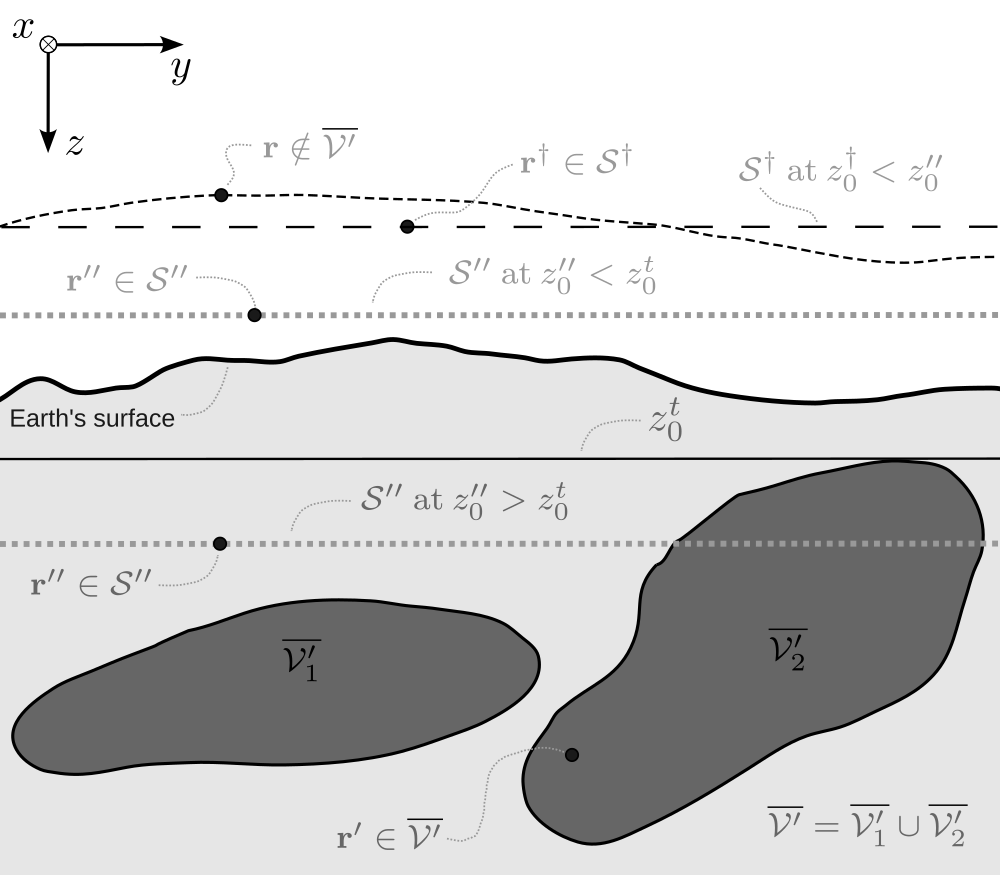
\includegraphics[width=0.8\textwidth]{Figure2_1.png}
	\caption{%
		2D schematic representation of a vertical $yz$ plane crossing the sources (represented in dark gray),
		with $x$ axis pointing inward the page (represented by the ``$\otimes$" symbol).
		The sources are located in the subsurface (represented in light gray), over a 
		closed region $\overline{\mathcal{V}'}$ with top limited by the plane $z^{t}_{0}$. 
		The fine dashed lines represent two possible horizontal surfaces $\mathcal{S}''$, one located 
		at $z''_{0} < z^{t}_{0}$, above the sources, and another at $z''_{0} > z^{t}_{0}$, crossing the sources.
		The medium dashed line represents the surface containing the observation points 
		$\mathbf{r}$, all above $\mathcal{S}''$.
		The long dashed line represents a planar surface $\mathcal{S}^{\dagger}$ located 
		at $z^{\dagger}_{0} < z''_{0}$.
	}
	\label{fig:Figure1}
\end{figure}